\subsection{Medjureprezentacija visokog nivoa (MVN) - High-Level Intermediate Representation (HIR)}

\subsubsection{Konstrukcija}

Obradom proširenog oblika apstraktnog sintaksnog stabla nastaje medjureprezentacija visokog nivoa.
Proces obrade se naziva snižavanje (\verb|lowering|). Neke sintaksne forme bivaju pojednostavljene.
Zagrade se uklanjaju jer struktura stabla eksplicitno odredjuje redosled operacija. \verb|For| petlje 
se konvertuju u \verb|while(let)| petlje \ref{lst:hir_iter}. Izraz \verb|if let| se prevodi 
u \verb|match| izraz. Izraz \verb|impl| u parametrima funkcije se konvertuje u generički argument.
Pojednostavljenje je način da se zaobidju granični slučajevi i smanji količina koda koja je potrebna 
da se izvorni kod analizira.

\begin{listing}[H]
\begin{minted}{rust}
// Pre
for elem in vec {
    process(elem);
}
// Posle
let mut iterator = vec.into_iter();
while let Some(elem) = iterator.next() {
    process(elem);
}
\end{minted}
\caption{"for" petlja pre i nakon pojednostavljenja}
\label{lst:hir_iter}
\end{listing}

\verb|Crate| je ponovo čvor najvišeg nova ali za razliku \verb|Crate|-a apstraktnog sintaksnog stabla koji sadrži
samo podatke o korenskom modulu, \verb|Crate| visoke medjureprezentacije skladišti sadržaj celokupnog paketa.
Izvorni kod koji se ne koristi niti implicitno niti ekplicitno nije postojan unutar ovog pogleda. Značaj 
ove osobine se najviše ispoljava prilikom upotrebe eksternih biblioteka, gde je uobičajno koristiti samo 
deo funkcionalnosti.

\subsubsection{Sitem upita}

\verb|HIR| je najkorišćeniji oblik izvornog koda u \verb|rustc| \verb|frontend|-u. Takodje je prvi oblik koji 
koristi sistem upita (\verb|query|) i od izuzetne je važnosti prilikom inkrementalnog kompajliranja.
Iz perspektive kompajlera znanje u vezi \verb|Crate|-a je baza podataka, dok su upiti način na koji 
se dobavljaju podaci. Naime ključna razlika izmedju standardne baze podataka i "baze podataka" kompajlera
to što "baza podataka" kompajlera počinje prazna i puni se kada se upiti izvrše. To znači da upit mora 
da zna kako da izračuna izlaz u slučaju da rezultat ne postoji u "bazi podataka". "Baza podataka" kompajlera 
se naziva kontekst upita.

Upit se identifikuje pomoću imena. Ključ specificira koji podatak treba da se dobavi i taj podatak 
mora da poseduje povratni tip. Provajder je funkcija koja specificira kako se računa rezultat ukoliko nije 
prethodno izračunat. Esencijalno, upit je funkcija koja mapira ključ na rezultat. 
Povratne vrednosti upita se keširaju. Povratna vrednost bilo kojeg suksesivnog upita sa istim parametarima rezultovaće 
kopiji već izračunate vrednosti unutar keša. Ovakva tehnika keširanja rezultata se naziva memoizacija.
Keširanje je neophodno da bi sistem upita bio efikasan. Bez njega iste kalkulacije bi se ponavljale proizvoljan broj puta.

Da bi ovaj sistem funkcionisao na prethodno opisan način uvode se pojedina pravila. Ključ i rezultat 
moraju biti nepromenljive vrednosti. Provajder mora biti deterministička funkcija, tj. upit za isti ključ
uvek vraća istu vrednost. Jedini parametri upita jesu ključ i konstekst kompajliranja (baza podataka).
Memoizacija je jedan od glavnih razloga za ova pravila. Ukoliko bi provajder mogao da vrati nedeterministički rezultat,
tačnost keširanjog rezultata ne bi mogla biti zagarantovana.

Pozivi upita moraju da kreiraju direkcioni aciklični graf. Pošto su provajderi samo obične funkcije lako je pretvoriti 
aciklični graf u ciklični dodavanjem funkcije koja kreira ciklus. Ranije je \verb|rustc| kompajler imao podršku 
za prekidanje ciklusa i nastavkom rada, ali teoretski takvo izvršavanje nije determinističko i nije zasigurno da bi 
inkrementalno kompajliranje radilo. Danas, sistem upita prijavljuje grešku da je pronadjen ciklus
i ne nastavlja sa kompajliranjem.

Rezultati upita mogu biti ukradeni, tj. rezultat se nalazi unutar strukture \verb|Steal<t>| i očekuje se da će se vlasništvo 
preneti ka nekom drugom kontekstu u nekom trenutku. Ova tehnika se primarno koristi zbog performansi, 
jer su neke vrednosti skupe za kloniranje. Ovaj postupak ne nanosi štetu u kontekstu inkrementalnog kompajliranja jer se pre 
prenosa vlasnišva izvršavaju svi upiti koji bi mogli da potraže ovaj rezultat. Sa obzirom da se upiti koji traže rezultat 
moraju navesti manuelno, prostor za grešku je veliki. Ukoliko je ukradeni rezultat potražen od nekog upita nakon što je preneto vlasništvo
kompajler prijavljuje grešku, osiguravajući bezbedno stanje.

\subsubsection{Inkrementalno kompajliranje}

Inkrementalno kompaljiranje se oslanja na strukturu direkcionog acikličnog grafa kroz "\verb|try|-\verb|mark|-\verb|green|" algoritam.
Ovaj algoritam potiče od "\verb|red|-\verb|green|" algoritma. Ideja je da nakon svakog upita se sačuva rezultat upita ali i direkcioni 
aciklični graf tog upita tj. rezultate upita koje je roditeljski upit pozvao. Prilikom suksesivnog pokretanja kompajlera potenicjalno 
je moguće iskoristiti rezultat nekih upita iz prethodne kompilacije. Ovo se postriže dodeljivanjem boje svakom upitu. Ako se rezultat 
upita promenio u odnosu na prethodni put, upit postaje crven. Ukoliko je rezultat isti kao i prethodni put, upit postaje zelen. 
Iz ovoga proizilaze dva nova pravila. Ako su svi ulazi u upit isti, onda će i rezultat upita biti isti. Ovim se spašava značajno vreme 
koje bi se inače potrošilo na čitanje i deserijalizovanje podataka sa diska. Nasuprot ovog pravila, ako se ulaz u upit promenio, 
a i dalje je vratio isti rezultat, upit se boji u zeleno i zaobilazi se ponavljanje ovog upita.

Algoritam "\verb|try|-\verb|mark|-\verb|green|" radi na sledeći način. Proverava da li je upit izvršen u prethodnoj kompilaciji. Ako 
nije, upit se evaluira i boji crvenom. Ako jeste, učitavaju se sva deca (zavisnosti) tog upita. Za svaku zavisnost upita rekurzivno 
evaluirati boju istim redosledom kao i u prethodnoj kompilaciji. Ukoliko su sve zavisnosti zelene onda je i roditeljski upit zelen.
Ako je bilo koji čvor u ovom procesu crven, roditeljski čvor je prljav. Izvršavaju se sve zavisnosti roditeljskog upita, a potom 
poredi heš rezultata sa heš-om prethodnog rezultata. Ako se heš nije promenio roditeljski upit postaje zelen, u suprotnom crven.

Lažno pozitivne vrednosti su problem prilikom upotrebe ovakvog algoritma. Pretpostavlja se da upit "odredi znak" postoji i da su 
ulazi početne i naredne kompilacije u ovaj upit redom brojevi 500 i 1000. Iako je očigledno da se znak nije promenio, kompajler 
mora biti konzervativan i ponovo evaluairati rezultat ovog upita.

Kada kompajler prestane sa radom, sve evaluirane vrednosti u memoriji bivaju uništene. Stoga rezultati upita moraju da se čuvaju 
na disku. Ovo dovodi do novih problema koji se moraju rešiti. Rezultati na disku nisu odmah spremni za poredjenje. Identifikatori 
čvorova grafa izmedju kompilacija su potencijalno pomereni (\verb|NodeId|, \verb|DefId|). Perzistiranje na disk ima svoju cenu i 
nije smisleno svaku sitnu informaciju čuvati na disku. 

Ukoliko se kod nije menjao i redosled definicija/implementacija u kodu ostao isti generisani 
identifikatori ostaju isti, ali ukoliko se bilo šta pomerilo ne postoji garancija da je i dalje tako. Ovaj problem se rešava 
uvodjenjem stabilnih formi identifikatora. Za najbitniji slučaj \verb|DefId| stabilna zamena je \verb|DefPath|. \verb|DefPath| nije numerički 
i oslanja se na putanju kao što je \verb|std::collections::HashMap|, čime nije afektovan nerelevantnim promenama u izvornom kodu. 
\verb|DefPathHash| je 128 bitna reprezentacija \verb|DefPath|. Praktično gledano, obe reprezentacije sadrže istu informaciju pa se 
\verb|DefPathHash| češće koristi jer je lakši za upotrebu. Prilikom deserijalizacije rezultata \verb|DefPathHash| se mapira na 
\verb|DefId| iz trenutne kompilacije. \verb|HirId| je identifikator komponenti visoke reprezentacije koje nemaju \verb|DefId|. 
\verb|HirId| je spoj \verb|DefPath| i \verb|LocalId|. \verb|LocalId| identifikuje izraz unutar neke stavke koda, na primer 
definicija varijable unutar funkcije.

Prilikom izvršavanja "\verb|try|-\verb|mark|-\verb|green|" algoritma često se poredi rezultat upita trenutne kompilacije u odnosu 
na rezultat upita u prethodnoj kompilaciji. Deserijalizacija rezultata sa diska je skupa operacija, a rezultat trenutnog upita je 
već sračunat i može da se koristi. Kompajler prevazilazi ovaj problem upotrebom otisaka prista (\verb|fingerprint|). Otisak prsta 
je 128 bitni heš rezultata upita. Jeftino je učitati celokupnu mapu otisaka prstiju prilikom učitavanja direkcionog acikličnog grafa 
i poredjenje se svodi na jeftino uporedjivanje rezultata iz mape. Verovatnoća da se kolizija heš vrednosti dogodi je izuzetno mala 
jer se koristi kvalitetan heš. Naime upotreba kvalitetnog heša dovodi da u nekim slučajevima inkrementalna kompilacija biva 
sporija od neinkrementalne usled vremena provedenog u računanju heš vrednosti. Otisci prstiju se koriste prilikom korelacije 
izmedju čvora prethodnog i trenutnog direkcionog acikličnog grafa, tako što se otisak prsta računa nad ključem upita.

Dešava se da neki čvorovi izmedju dve kompilacije ne budu evaluirani jer su čvorovi samo zavisnosti roditelja koji je obojen 
zelenom. Prateći prethodno opisan algoritam dobilo bi se da novi direkcioni aciklični graf ne sadrži više ove zavisnosti. Zbog 
toga se primenjuje promocija keša. Pre nego što se rezultat inkrementalne kompilacije prebaci na disk, izvršiće se prolazak 
kroz sve zavisonosti svakog zelenog čvora i postaraće se da su učitani u memoriju. Na ovaj način zavisnosti koje trenutno 
nisu možda neophodne mogu biti iskorišćene u budućim kompilacijama. 

Upiti mogu da sadrže modifikatore koji utiču na to kako se sistem upita ophodi prema upitu prilikom inkrementalne kompilacije.
Modifikator \verb|eval_always| označava da upiti nikada neće biti zelen i preskače se prilikom "\verb|try|-\verb|mark|-\verb|green|".
Ovaj modifikator je koristan u slučaju da upit čita vrednost iz nekog fajla ili globalnog stanja gde može doći do mutacija. Takodje neki 
upiti zavise od celokupnog izvornog koda i nema potrebe pokušavati keširati rezultat jer će uvek boja biti crvena. Modifikator 
\verb|no_hash| označava da za upit nikada neće biti računat otisak prsta. Iz ovoga sledi da svaki upit koji zavisi od \verb|no_hash|
upita mora biti rekalkulisan. Ovaj modifikator je koristan u slučaju kada bi se otisak prsta računao nad velikim i kompleksnim 
vrednostima gde bi ovaj postupak trajao dugo. Takodje za funkcije koje su veoma osetljive na promene upita (a * b * c), promena 
ulaza će skoro uvek rezultovati crvenoj boji čvora. Modifikator \verb|cache_on_disk_if| odredjuje da li će rezultat upita biti 
sačuvan na disku. 

Modifikatori \verb|eval_always| i \verb|no_hash| mogu biti zajedno korišćeni u šablonu koji se naziva projekcionim upiti. Postoje upiti koji zahtevaju 
celokupan ulaz kompajlera (indeksiran \verb|HIR|). Ovakvi upiti se često modeluju tako što se veliki upit makira sa \verb|eval_always|
da bi se sačuvalo vreme. Zavisnosti upita (projekcije) su upiti koje zasebno mogu biti obojene crveno ili zeleno. Time se omogućava 
da neke projekcije budu crvene i evaluirana ponovo dok ostale zelene projekcije mogu da iskoriste prethodni rezultat.

\begin{listing}[H]
\begin{center}
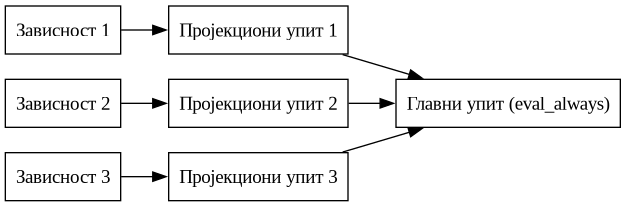
\includegraphics[width=4in, height=1.6in]{assets/images/projection_query.png}
\end{center}
\caption{Upotreba "eval\_always" modifikatora u projekcionom šablonu}
\label{lst:projection_query}
\end{listing}